

\chapter{Findings}
\section{Possible Path Traversal of Apache Server on port 80}
\hrule
\begin{table}[htb]
    \renewcommand{\arraystretch}{1.5}
    \begin{tabular*}{\textwidth}{|>{\columncolor{orange!15}}p{3cm}|p{17.2cm}|}
    \textbf{Finding} & \textbf{Possible Path Traversal of Apache Server on port 80}\\
    Risk& Medium\\
    Category&Access Controls\\
    Impact& An attacker could access sensitive data. This can also happen with any user by accident. \\ \\
    Description& After performing an nmap scan three open ports where found. Since there is most likely a \ac{http} service running on port 80 a http-enum script was used to try to access several potentially interesting paths.
    \newline
    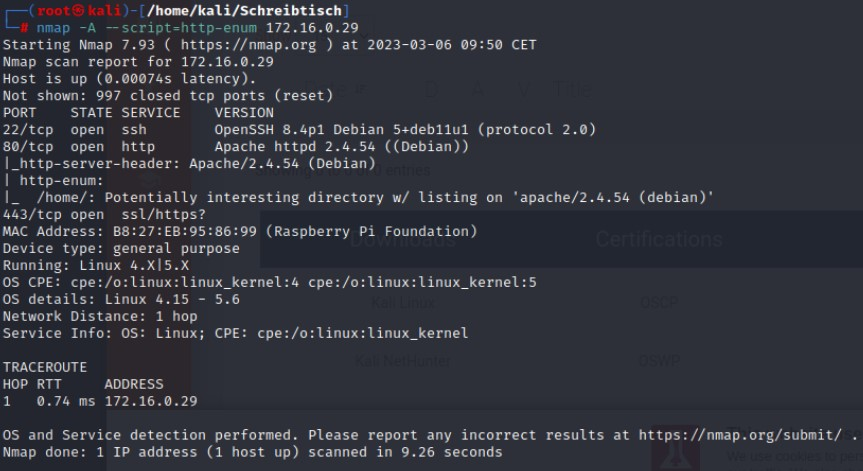
\includegraphics[width = 0.73\textwidth]{http_vulnerbility.jpg}
    \newline
    The script was able to access the ''/home'' path where the apache server has its directories saved. In this case no sensitive files were found. 
    \\&
    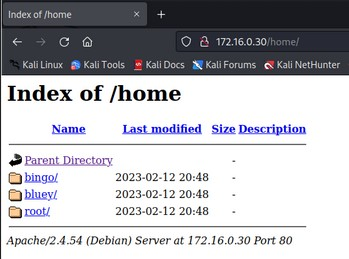
\includegraphics[width = 0.5\textwidth]{dateisystem.jpg} \\
    &\\
    \end{tabular*}
    \end{table}

    \newpage
    \begin{table}[htb]
    \renewcommand{\arraystretch}{1.5}
    \begin{tabular*}{\textwidth}{|>{\columncolor{orange!15}}p{3cm}|p{17.2cm}|}
    \textbf{Finding} & \textbf{Possible Path Traversal of Apache Server on port 80}\\
    Recommendation& Ensure that users can only access paths they are supposed to. This could be done by requesting a password if someone tries to access the website or implement a login system where users have to login first to access the path. \\    
    \end{tabular*}
    \end{table}